\documentclass[11pt,a4paper,titlepage]{article}

\usepackage[spanish,es-nodecimaldot]{babel}
\usepackage[utf8]{inputenc}
\usepackage[T1]{fontenc}
\usepackage[margin=0.9in]{geometry}
\usepackage{amsmath,amsfonts,graphicx,float,booktabs,url,siunitx,mathrsfs,tensor,wrapfig}
\usepackage[font=footnotesize,labelfont={sf,bf},textfont=sf]{caption}
\usepackage[usenames,dvipsnames]{xcolor}
\usepackage[plainpages=false,pdfpagelabels,hypertexnames=false,hidelinks]{hyperref}
\graphicspath{{./Img/}}
\captionsetup{width=0.7\linewidth}

\makeatletter
\DeclareMathSizes{\@xpt}{\@xpt}{6}{5}
\makeatother

\title{\Huge\textbf{El problema de la cuantización de la interacción gravitatoria}}
\author{\textsf{Iyán Méndez Veiga}\\ \textsf{Víctor Rodríguez Bouza}}
\date{\texttt{TRG 2015-2016}}

\newcommand{\HRule}{\rule{\linewidth}{0.5mm}} % Para el título

\addto{\captionsspanish}{\renewcommand{\refname}{\vskip -1cm}} % Para que BibTeX no ponga su título propio.
\setlength{\parskip}{1em} % Cambia aquí la separación a la que te guste pero lo de usar \\ + \par es mala práctica, a mí me salen todos warnings con underfull y tal

% -------------------------------------------------------------

\begin{document}
%
%
%
%
\begin{titlepage}
\begin{titlepage}
\begin{center}

% Upper part of the page. The '~' is needed because \\
% only works if a paragraph has started.

% Title
\HRule \\[0.4cm]
{ \huge \bfseries El problema de la cuantización\\de la interacción gravitatoria. \\[0.3cm] }

\HRule \\[1.5cm]

\textsc{\Large Teoría de la Relatividad General}\\[1cm]

\vfill

% Bottom of the page
\large{\textsf{Iyán Méndez Veiga y Víctor Rodríguez Bouza}}


\textmd{Facultad de Ciencias \\
Universidad de Oviedo}

\texttt{Curso 2015-2016}



\end{center}
\end{titlepage}

\end{titlepage}
%
%
%
%
%\newpage
%\setcounter{page}{2}
%\thispagestyle{empty}
%\mbox{}
%
%
%
%
\newpage
\tableofcontents
\newpage
%
%
%
%
%\newpage
%\setcounter{page}{4}
%\thispagestyle{empty}
%\mbox{}
%
%
%
%
\begin{abstract}
La fuerza gravitatoria es una de las cuatro interacciones que gobiernan el universo. Durante todo el siglo XX, los modelos de la misma han recibido un empujón gracias a la teoría de la relatividad general de Albert Einstein, pero diversos problemas han aflorado a finales de la centuria. En tal situación, la cuantización de la gravedad se hace necesaria. En este trabajo explicamos los motivos por los que los investigadores de finales de siglo se ven obligados a tal esfuerzo. A continuación, explicamos la esencia de las principales alternativas que están en estudio para resolver el problema: \textit{Loop Quantum Gravity}, teoría de cuerdas, o aproximaciones covariantes entre otras. Finalmente exponemos las últimas novedades en el campo, unas conclusiones de más de medio siglo cuantizando la gravedad y las perspectivas futuras.
\end{abstract}
%
%
%
%
\section{Introducción. ¿Por qué es necesaria la cuantización de la gravedad?} % Víctor

\subsection{Aproximación histórica}

Para los antiguos astrónomos, el cielo estrellado escondía misterios que les apasionaban. ¿Por qué el Sol, que tanto calor nos da, y permite a nuestros cultivos florecer, aparece al amanecer y se esfuma al atardecer? ¿Qué son las estrellas? ¿Luces «pegadas» sobre una esfera perfecta, como diría Aristóteles? ¿O algo más? ¿Hay gente acaso viviendo en las estrellas? ¿Podemos ir a la Luna? Obviamente, la bóveda celeste era una fuente casi inagotable de inspiración: origen de multitud de leyendas y narraciones mitológicas.

\begin{wrapfigure}{r}{0.45\textwidth}
	\centering
	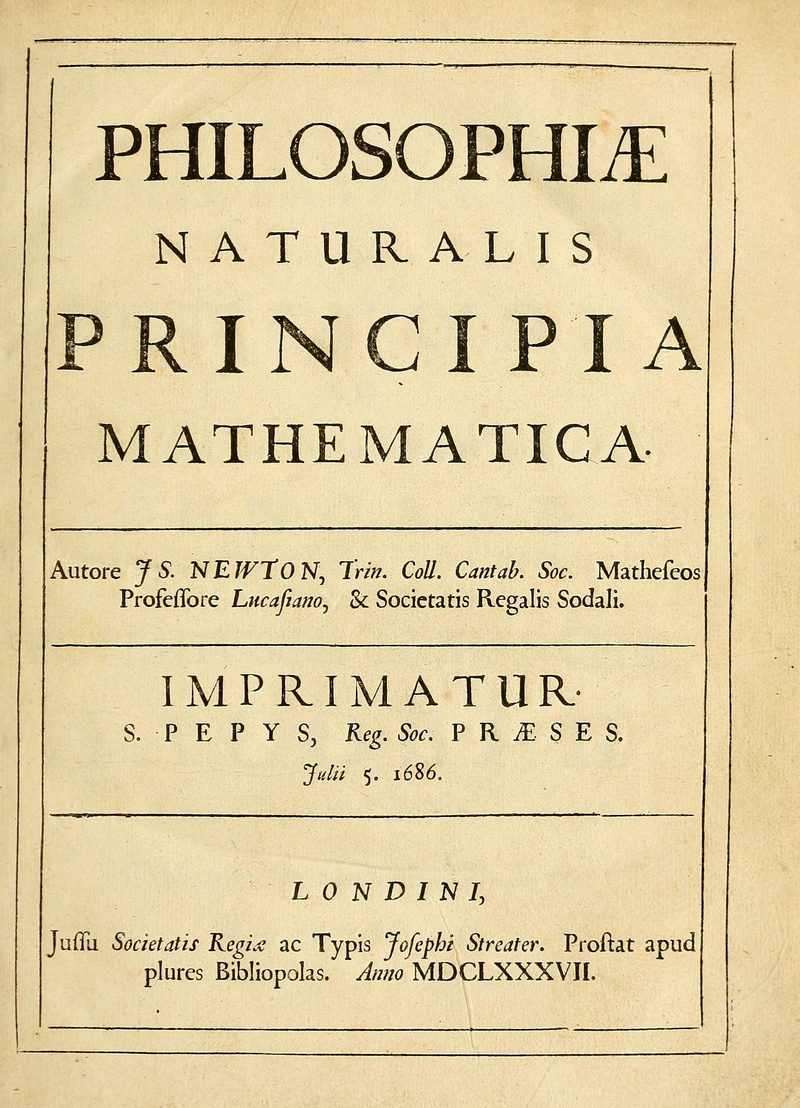
\includegraphics[width=0.45\textwidth]{newton}
	\caption{\cite{newtonbib}.Portada original de los \textit{Philosophiae Naturalis Principia Mathematica}, la obra más importante de Newton en la que describe su nueva concepción de la mecánica que revolucionaría la percepción científica de la humanidad.}
	\label{fig:newton}
\end{wrapfigure}

Uno de los procesos que ya intrigaba en la antigüedad eran los movimientos de cuerpos como Marte u otros, que eran \textit{erráticos} (¡el que menos!). Como es bien sabido, la evolución de la investigación en estos campos derivó en distintas concepciones de distribución de los astros en el cosmos. Aristóteles, Ptolomeo y otros ofrecieron sus propuestas respecto al por qué de estos movimientos. Sería más adelante, durante la Revolución Científica del Renacimiento cuando el modelo heliocéntrico de Aristarco rescatado por Copérnico se asentara firmemente, sobre todo en el siglo XVII. \textbf{Kepler} fue el primero que dio un análisis físico (en el sentido que hoy lo consideraríamos) sobre el movimiento de los cuerpos del sistema solar. Sin embargo, la humanidad tuvo que esperar algunos años más para que llegara la primera concepción científica (en el sentido actual) sobre la fuerza que origina tales desplazamientos: \textbf{la gravedad}.

\textit{Sir} Isaac Newton ofreció en el siglo XVII un modelo matemático de lo que bautizó como fuerza gravitatoria, basado en su cálculo de fluxiones (cálculo diferencial) y la idea mejorada del movimiento galileano. Ésta interpretación es considerada como la proposición de Newton para los modelos sobre gravedad en la «concepción clásica de la física». Es esencialmente lo que hoy en día se entiende por \textbf{gravedad newtoniana}.

Éste modelo de fuerza gravitatoria permitió entender esta interacción tanto en cuerpos diminutos, como en planetas y estrellas muy masivas. Habilitó la posibilidad de avance del estudio de la mecánica celeste, interpretando las leyes de Kepler como particularizaciones de su modelo y cosechando numerosos éxitos experimentales. Un ejemplo es el descubrimiento de Neptuno, que se hizo tras haberse hallado perturbaciones en el período de la órbita de Urano. Entonces, Urbain Le Verrier predijo la existencia de un nuevo planeta, empleando la teoría de Newton. Tal cuerpo afectaría a la órbita de Urano y permitiría explicar tales órbitas. Su colega Gottfried Galle descubriría más tarde a Neptuno tal y como Le Verrier había dicho.

Pero no sería la única órbita que se escapara a las predicciones iniciales de la gravedad newtoniana. El propio Le Verrier descubrió que, pese incluso contando con la acción del resto de planetas (además del Sol) sobre el planeta Mercurio, había extraños resultados experimentales en su órbita que no cuajaban con las predicciones newtonianas, concretamente, su precesión en el perihelio. En un alarde de innovación, Le Verrier, basándose en que la teoría de Newton era correcta, propuso en 1859 la hipótesis de un nuevo planeta entre Mercurio y el Sol: Vulcano. Sin embargo, éste nunca se descubrió.

\begin{wrapfigure}{l}{0.40\textwidth}
	\centering
	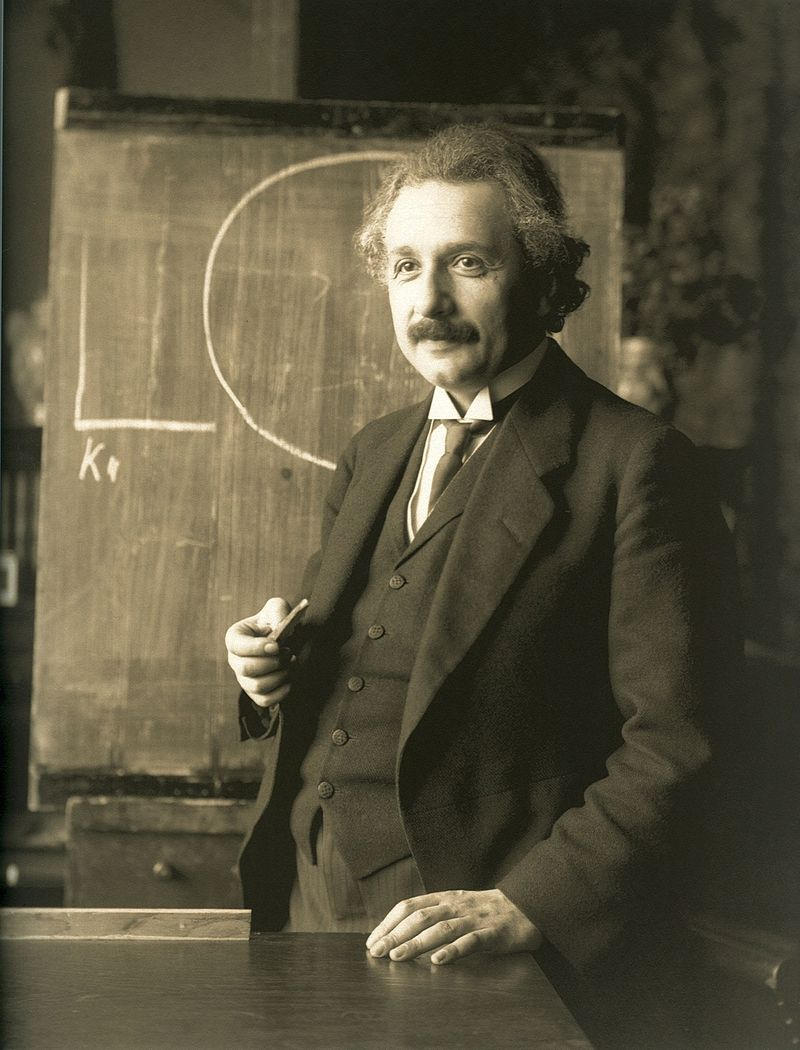
\includegraphics[width=0.40\textwidth]{einstein}
	\caption{\cite{einsteinbib}. Albert Einstein (1879-1955) fue uno de los más relevantes científicos del siglo XX y de la humanidad. Su trabajo de las teorías de la relatividad especial y general modificaron cualitativamente la percepción de la realidad. Cabe decir que antes de que Einstein presentara su artículo, Hilbert llegó a dar con una ley de gravitación completamente igual a la del primero de forma independiente. La publicación el 25 de noviembre de 1915 en la Academia Prusiana de Ciencias por parte de Einstein de sus resultados generó una situación incómoda entre ambos. Sin embargo, Hilbert acabó aceptando lo sucedido, y cedió todo el protagonismo a Einstein en su obra maestra. En el futuro, Einstein y Hilbert se considerarían el uno al otro como colegas científicos, sin recuerdo de esos «nubarrones» (\cite[p.~49-50]{teoriaperfecta}).}
	\label{fig:einstein}
\end{wrapfigure}

Albert Einstein trabajaba en una oficina de patentes en Berna (Suiza) cuando postuló su teoría de la relatividad especial. Debido a su trabajo monótono y repetitivo, podía abstraerse en el mismo y hacer experimentos mentales físicos (\textit{Gedankenexperiment} o \textit{Gedankenversuch}) para poner a prueba sus ideas . Cuando se dedicó a hacer compatible la teoría de la relatividad especial con la gravedad newtoniana se dio cuenta de numerosas problemáticas que lo forzaron a desarrollar un nuevo marco en los comienzos del siglo XX para la interacción gravitatoria. Un marco no cuántico, pero que sí incluyera la relatividad especial y la gravedad clásica. Dicho modelo acabaría llevando el nombre de \textbf{teoría de la relatividad general}.

Como teoría científica que se precie, debía poder ponerse a prueba, y así fue. Una de las comprobaciones de su utilidad está en que con este modelo es posible interpretar el extraño fenómeno de la órbita de Mercurio, por ejemplo. Otras pruebas de la teoría, como la observación de estrellas tras el Sol durante un eclipse, confirmaron su validez.


Las ecuaciones de Einstein (como se conoce a las principales relaciones de éste modelo) son una herramienta muy potente para entender el funcionamiento general del cosmos. Y muy liosa, también. Einstein fue, obviamente, el primero que se lanzó al empeño de resolverlas, buscando un \textbf{modelo adecuado} de la realidad que nos rodea surgido de ellas. El resultado al que llegó fue una solución en la que aplicó el conocimiento (muy limitado para nosotros) que en 1916 se tenía del universo cercano: supuso que el universo estaba repleto de masa distribuida de forma uniforme. Dadas esas hipótesis, llegó al extraño resultado de que tal universo debería empezar eventualmente un proceso de evolución, de cambio, de modo que en un determinado momento, el universo no siguiera siendo estático a escala macrocósmica. Esta posibilidad fue despreciada por Einstein, quien derrotado por su intuición física y sus ideas preconcebidas \textbf{introdujo una constante en las ecuaciones} cuyo único fin era contrarrestar los efectos de la masa sola en el universo. De este modo, se podía tener un universo estable, en un equilibrio entre las fuerzas de la masa del mismo y lo que las contrarrestaba la constante.

Dicho valor recibió el nombre de \textbf{constante cosmológica} y es uno de los pilares hoy en día de la cosmología moderna. Pero, ¿qué es la cosmología en esencia? La cosmología, en su acepción científica, es una disciplina dependiente de la física que estudia el origen, evolución y destino del universo en su totalidad empleando modelos físicos para tal fin. Será durante el siglo XX cuando recibirá su impulso principal, gracias a la teoría de la relatividad general.

En los años siguientes numerosos modelos surgieron a raíz de las conocidas como ecuaciones de Einstein: el modelo De Sitter, el de Lemaître, el de Friedmann, etcétera. Las pruebas experimentales acabaron demostrando, a través del corrimiento al rojo (o \textit{redshift}) que \textbf{el universo no es estático y} que \textbf{se encuentra en expansión} gracias a Hubble, Ryle y otros que rebatieron las tesis estacionarias de Hoyle y compañía.

\begin{wrapfigure}{r}{0.44\textwidth}
	\centering
	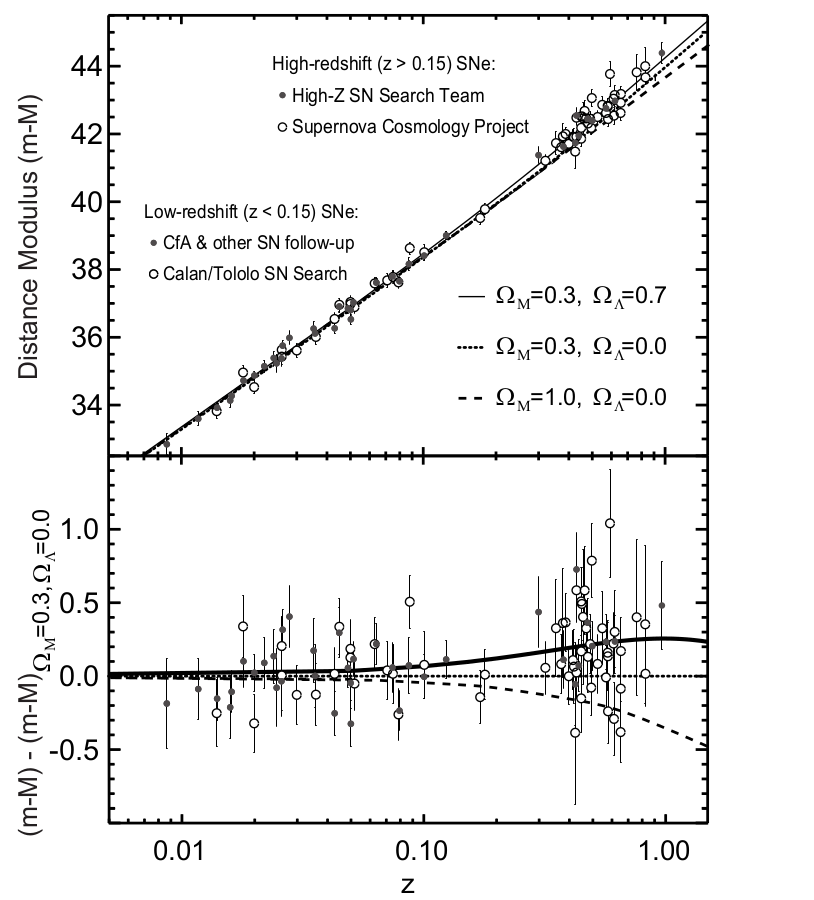
\includegraphics[width=0.44\textwidth]{hubble2}
	\caption{\cite[p.~17]{perlmutterschmidt}. Resultados experimentales de cosmología observacional con supernovas de tipo Ia que confirmaron la expansión del universo (predicha por Hubble) y la aceleración.}
	\label{fig:einstein2}
\end{wrapfigure}

A lo largo de lo que quedaba del siglo XX, los estudios sobre relatividad general aumentaron, tratando temas muy diversos: el Big Bang y la evolución hasta nuestros días, búsqueda de otras pruebas experimentales (como ondas gravitacionales), temas relacionados con materia oscura o energía oscura o incluso surgieron algunos problemas que apuntarían a una posible cuantización de la teoría para solventarlos (empresa que hoy en día sigue). Podríamos estar discutiendo durante muchos párrafos todo ésto, pero ese no es el fin de este texto.

En 1947, y justo al acabar la carrera, \textbf{Bryce DeWitt} tuvo la oportunidad de conocer a Wolfang Pauli, aprovechando la ocasión para decirle que \textbf{estaba trabajando en la cuantización del campo gravitatorio}. A DeWitt le resultaba incomprensible que las dos teorías científicas más revolucionarias del siglo XX (la física cuántica y la relatividad general) no tuvieran ninguna relación entre sí. Pauli, sin embargo, no estaba de acuerdo con que DeWitt empleara su tiempo en ello: «ese problemas al que apuntas es muy importante, pero para resolverlo se necesitará a alguien realmente listo»\footnote{\cite[p.~230]{teoriaperfecta}.}. Sin menoscabo de la inteligencia o de la capacidad de DeWitt, el tiempo ha demostrado lo acertado que estaba Pauli.

Los primeros pasos hacia tal hipotético encuentro entre Einstein y la mecánica cuántica los daría Paul Dirac. Sería él, quien junto a otros como Klein-Gordon propiciaran el advenimiento de la \textbf{teoría cuántica de campos} (\textit{Quantum Field Theory} o QFT) gracias a la ecuación de Dirac. Ésto posibilitó (además de otras importantes contribuciones) reencontrar las nuevas teorías sobre partículas con la relatividad especial de Einstein, acercándolas a la relatividad general un poco más.

Quiere ser la historia irónica, y el hecho es que a Dirac las nuevas teorías de física de partículas que acabarían dando el hoy famoso modelo estándar (\textit{Standard Model}, SM) no le gustaban ni un pelo. Pese a agregar a las fuerzas débil y fuerte, y ofrecer predicciones que se mostrarían certeras, lo que incordiaba a Dirac era la «suciedad formal» que tenía la teoría en forma de \textit{renormalizaciones}. Dirac era un hombre que apreciaba lo matemático, las relaciones, la realidad que subyacía a los experimentos mundanos de laboratorio.

En los últimos años de su vida, Dirac acabó aislado de la comunidad científica por su negativa a aceptar los logros de la física cuántica. No cesó de instigar a sus compañeros a buscar una teoría más general que no necesitara de las \textit{abyectas} renormalizaciones. Tampoco le sorprendió nada que DeWitt, eventualmente hallara problemas de renormalización en su cuantización de la gravedad. Dirac creía que para unificar ambos mundos sería necesaria una comprensión más profunda de la teoría cuántica.

DeWitt, mientras, se dedicó a intentar cuantizar el gravitón, que sería la partícula que «transportaría» (mediaría) la interacción gravitatoria: empresa más ardua de las que nunca imaginara, y que ya habían intentado otros como Matvei Bronstein, el propio Paul Dirac, Richard Feynman, Wolfgang Pauli o Werner Heisenberg. Los esfuerzos que él y otros a la par como Dennis Sciama (Óxford), Stanley Deser (Boston) o Abdus Salam (Paquistán) estaban llevando a cabo se pusieron en común en 1974, cuando se realizó un simposio sobre gravedad cuántica en la Universidad de Óxford.

Aunque la comunidad científica vivía una relativa euforia (el ya existente CERN no paraba de confirmar los resultados que el modelo estándar de física de partículas predecía), según fueron pasando los ponentes ese clima de éxtasis se fue esfumando. De acuerdo con Wolfgang Pauli, se podía escuchar cómo los organizadores del evento murmuraban inquietos: «lo que Dios ha separado, que no lo una el hombre»\footnote{\cite[p.~242]{teoriaperfecta}.}.

La gravedad cuántica parecía estar en un callejón sin salida y la reconciliación de la fuerza gravitatoria con las otras tres parecía imposible, y el simposio de Óxford fue la viva imagen de ello... en su \textit{inmensa} mayoría. El evento habría significado la viva imagen de la derrota de no ser por la conferencia que diera el científico de la Universidad de Cambridge \textbf{Stephen Hawking}. Sería éste quien mostrara un vínculo entre la gravedad de Einstein y la física cuántica a través de un \textbf{modelo de los agujeros negros}.

Lo que se descubrió, en resumen, en las postrimerías del siglo XX fueron una serie de problemas que aparecían con la relatividad general cuando se las aplicaba a algunos casos \textit{extremos}. Un ejemplo de éstos casos podría ser mismamente el agujero negro. De este modo sería que la comunidad científica vería como necesaria la cuantización de la gravedad como solución a bastantes de ellos. También existen alternativas \textit{clásicas} de relatividad general, que intentan bordear problemas como la materia oscura o la energía oscura. Ejemplos de ellas son las MOND o TeVeS, pero no son objeto de estudio de este texto.

En este momento, resulta más adecuado para los fines del trabajo abandonar la perspectiva histórica y abordar los problemas de la relatividad general y la necesidad de la cuantización desde un punto de vista más \textit{aislado}. Veámoslo.


\subsection{La necesidad de la gravedad cuántica}
\par Como vimos en el epígrafe anterior, un conjunto de problemáticas y motivos empezaron a surgir a finales del siglo pasado que apuntaban a la necesidad de una teoría cuántica de la gravedad. En este apartado veremos cuáles han sido los principales argumentos que han sido esgrimidos hasta la actualidad para ello.

\begin{description}
  \item[Completitud formal.]{Como dijimos en el subapartado histórico, uno de los principales motivos para la búsqueda de una teoría \textit{superior} (entendiendo por ello que contenga a ambas) a la teoría de la relatividad general y la mecánica cuántica es la «completitud formal». Por ésto entendemos que la existencia de dos teorías con una confirmación experimental tan reafirmada como la gravedad de Einstein y la física cuántica y de aplicación al universo entero incita a pensar en su posible vínculo. Sería algo parecido a la motivación de DeWitt.

  Pero no es necesario quedarnos con esa idea tan abstracta del motivo: es muy sencillo encontrar experimentos mentales, como los usados normalmente en mecánica cuántica, para ver un posible vínculo. Veamos un ejemplo postulado por Feynman en la conferencia de Chapel Hill de 1957.

  Imaginemos una suerte de experimento de Stern-Gerlach en el que conseguimos eventualmente dos partículas en un estado de superposición de espín $+1/2$ y $-1/2$. Hagamos ahora pasar esas dos partículas por dos contadores (algo que las partículas puedan accionar), de modo que uno de ellos esté conectado a una bola de dimensiones macroscópicas que se mueva al activarlos. En tal caso, la superposición de las partículas será transferida a la bola, que podrá estar en dos posiciones distintas a la vez... pero esto quiere decir que el \textit{campo gravitatorio está en una superposición} también. Si hacemos que el campo de esa bola afecte a otras mayores o más distantes, para comprender la interacción gravitatoria de éstas deberemos seguir la cadena de fuerzas e interpretar en última instancia de un modo mecano-cuántico el campo gravitatorio.\footnote{Cabe resaltar que una comprobación experimental de estos «juegos mentales» no existe, pero sirven para expandir el campo de conocimiento y buscar una teoría más «completa». Así es en parte cómo avanza la ciencia.}}

  \item[Unificación.]{Las teorías de unificación de las interpretaciones de las fuerzas han resultado muy útiles en física de partículas, llevando a resultados experimentales muy contrastables. Haciendo la extensión, parecería lógico pensar que podría llegar a conocerse una teoría más general que incluyera las cuatro interacciones fundamentales, y tal modelo necesitaría de la cuantización del campo gravitatorio.}

  \item[Existencia de singularidades.]{En el electromagnetismo clásico se suelen dar singularidades (es decir, puntos donde los campos o determinadas funciones \textit{no existen}) que han sido resueltas en la electrodinámica cuántica. Cabría esperar que las singularidades de la teoría de la relatividad general (Big Bang, agujeros negros...) se pudieran resolver en una teoría cuántica de la gravedad.}

  \item[El problema del tiempo.]{Aunque tanto la gravedad de Einstein como las teorías cuánticas ofrecen resultados experimentales veraces, poseen una concepción de tiempo completamente distinta. En la mecánica cuántica, el tiempo se considera absoluto algo que con la incorporación de la rel. especial cambió: en teoría cuántica de campos es el espaciotiempo el que es absoluto. Sin embargo, ninguna de las dos tiene en cuenta las dilataciones temporales debidas al cambio del espaciotiempo por la masa-energía. Obviamente, ambas interpretaciones no pueden ser ciertas a la vez, y se hace necesaria una interpretación más general que esclarezca la problemática. Al hecho de que esta hipotética teoría no dependa de un tiempo \textit{fijo} se le suele llamar «independencia del fondo» o «\textbf{\textit{background independence}}».}

  \item[Incompletitud del modelo estándar.]{El \textit{Standard Model} ha sido uno de los mayores logros de la física desde mediados del siglo XX. Sin embargo, no es una teoría científica como la mecánica cuántica: es una explicación parcial de las interacciones entre partículas que no pretende ser una teoría completa. Es decir, una \textit{aproximación} a unas leyes generales que subyacen a los fenómenos y que permitirían una explicación más simple y mejor globalmente que la que ofrece el SM. Ésto no quita para que haya hecho predicciones maravillosas que han podido ser fantásticamente contrastadas, ni tampoco es posible quitarle relevancia a que ha sido capaz de dar una interpretación para tres de las cuatro fuerzas fundamentales.

  Una de las carencias del modelo estándar es que no es válido a energías arbitrariamente elevadas. Si éstas son altas, el modelo estándar deja de ser una teoría cuántica de campos consistente, debido a varios motivos (polos de Landau, inestabilidad del potencial efectivo, etcétera). No es lo único: tampoco se entiende la masa del bosón de Higgs, la cual debería ser considerablemente mayor.

  En este contexto es natural plantearse si estas carencias a tal régimen de energías no serán debidas a la ausencia de la interacción gravitatoria en el modelo, aparte de otras explicaciones (como las teorías de supersimetría, por ejemplo). Concretamente, se espera que la hipotética influencia de la gravedad en el modelo estándar ocurra a energías elevadas, cercanas a las de la escala de Planck ($l_P\sim\SI{1.6e-33}{cm}$, $t_P\sim\SI{5.4e-44}{s}$ y $m_P\sim\SI{1.2e19}{GeV.c^{-2}}=\SI{2.2e-5}{g}$). Debido a que el SM es una teoría \textit{cuántica} de campos, necesitaríamos cuantizar la gravedad de Einstein para introducirla en el mismo.

  Cabe destacar que la lejanía de los regímenes de energías que hemos citado son un bache para el avance de la gravedad cuántica, ya que se encuentran lejos de nuestras posibilidades factibles hoy en día. Tampoco tenemos un acceso «fácil» a fenómenos astrofísicos en los efectos de la cuantización se pudieran apreciar. Esto complica mucho la búsqueda de tal teoría, puesto que no se tienen resultados experimentales «gravitocuánticos» disponibles que sean precisamente los que tengamos que interpretar.}
\end{description}

\begin{figure}[h]
	\centering
	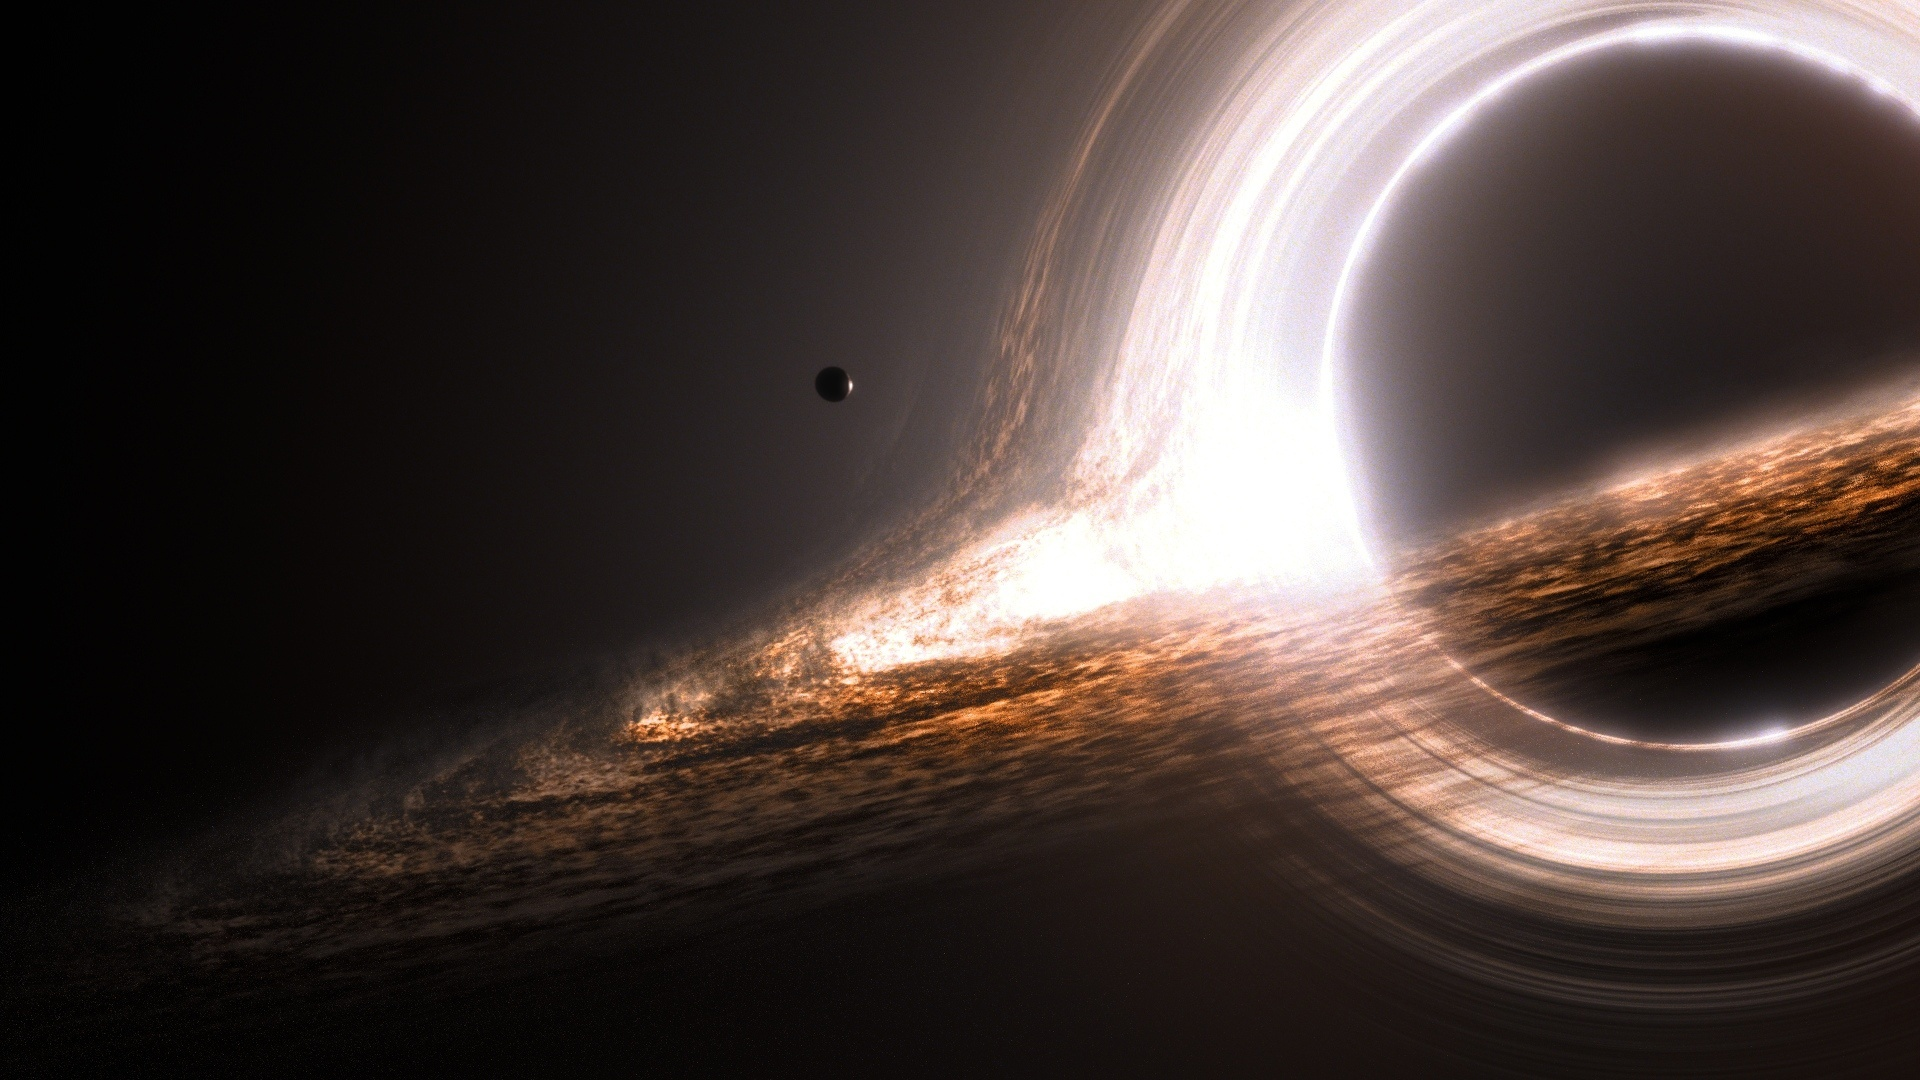
\includegraphics[width=0.8\textwidth]{interstellar}
	\caption{\cite{interstellarbib}. Fotograma del largometraje \textit{Interstellar} (todos los derechos reservados), en el cual se aprecia un agujero negro ficticio, Gargantúa. La recreación del fenómeno se realizó a partir de modelos físicos y simulaciones numéricas de los mismos.}
	\label{interstellarbib}
\end{figure}

\begin{description}
  \item[Existencia de resultados semiclásicos.]{Otro motivo viene de las aproximaciones a la teoría cuántica de la gravedad que se han venido haciendo, como la interpretación de Hawking de la temperatura de los agujeros negros (efecto Hawking). Pese a no tener comprobación empírica, resulta ilusionador que existan resultados basados en teoría cuántica de campos en espaciotiempos curvos que necesiten de ésta, de la mecánica cuántica, tengan una hipotética explicación. Además, ofrecen a nuestros colegas experimentales un reto: la medición de tales posibles predicciones. Que haya este tipo de modelos físicos es otro motivo más que incentive la búsqueda de una interpretación general que una los mundos cuántico y de la relatividad general.

  Uno de los ejemplos más característicos, como ya hemos dicho, es la interpretación de Hawking de los agujeros negros. Bajo la teoría cuántica de camos en un espaciotiempo curvo (o en un espaciotiempo plano, pero en un sistema de referencia no inercial), Hawking consiguió deducir que los agujeros negros necesariamente tenían una temperatura, y que por tanto también tenían una entropía (conocida como entropía de Bekenstein-Hawking), y una vida media. Ésto causó bastante conmoción en el simposio de Óxford en el cual el físico de Cambridge dio a conocer sus resultados. Conmoción, e incredulidad.

  El modelo de los agujeros negros de Hawking da parámetros que podrían ser eventualmente medidos en experimentos observacionales. Sin embargo, estamos lejos de acercarnos a tal suceso. Algunos investigadores apuntan a que la temperatura de los agujeros negros del comienzo del universo debería ser lo suficientemente alta como para que podamos medir su radiación.

  Cuando nos movemos a una situación en la que el agujero negro se hace pequeño, la interpretación de Hawking se desmorona, originando el conocido como \textbf{problema de la pérdida de información} (o \textit{information-loss problem}). La comunidad científica espera que una teoría cuántica de la gravedad propiamente dicha pueda resolverlo.

  Básicamente, el dilema se reduce a qué ocurre en el final de la vida del agujero negro. Si sólo quedara energía termal, entonces toda la información cuántica que entró en el agujero negro sería devuelta como un solo estado. Un solo estado de radiación térmica, es decir, un último estado de fotones. De este modo, la información sobre el estado inicial del agujero negro y toda aquella que hubiera atravesado su horizonte de sucesos se habría perdido, lo cual está en contradicción con la teoría cuántica para un sistema cerrado. Aunque no existe un consenso firme, parece que es posible ver que para un agujero negro semiclásico el problema no existe, aunque habría que considerar dentro del sistema el entorno del agujero negro.\footnote{\cite[p.~4]{paper_osorio}.}

  Sin embargo, las dudas siguen, y no sólo con el problema de la pérdida de información, sino con inconvenientes de la singularidad como lo que ocurre en el horizonte de sucesos de forma cuántica, o qué pasaría si un agujero negro se acercara a la escala de Planck. Todo ello no hace sino incentivar la búsqueda de una teoría cuántica de la gravedad.}

\end{description}

Como vemos, la ciencia ha encontrado motivos más que suficientes para emprender la búsqueda de una nueva teoría que explique la interacción gravitatoria de forma cuántica. Por desgracia, el universo es caprichoso y querrá ésta que no sea tan sencillo como con el resto de fuerzas esta empresa.
%
%
%
%
\newpage
\section{Los problemas de la cuantización}
Cuando los científicos (como DeWitt cuando terminó su licenciatura) se pusieron manos a la obra, no sabían lo que les venía encima. Quizás algunos pensaran que sería como cuantizar el electromagnetismo, como en QED. ¿Qué era lo que se había hecho para cuantizar el electromagnetismo? Emplear teoría cuántica de campos. Como ya dijimos en la introducción histórica, sería Dirac uno de sus mayores contribuidores de este estudio que revolucionaría la física. Sobre todo, la de partículas: es gracias a la QFT que el modelo estándar existe.

Una característica esencial de la teoría cuántica de campos (que, recordemos, aunaba relatividad especial y física cuántica en un único marco) es que es una \textbf{teoría perturbativa}. Ésto quiere decir que, para el cálculo de ciertos objetos emplea la teoría de perturbaciones de la mecánica cuántica: es decir, calcula por ejemplo hamiltonianos a través de una serie de potencias de un determinado parámetro, llamémoslo $\lambda$. Las «perturbaciones» vienen aquí de que, según cómo sea el susodicho $\lambda$, podemos despreciar la mayoría de los términos, quedándonos con el primero (que será el que tenga la potencia $\lambda^0$). Ésta aproximación válida para bajos $\lambda$ se asignaría a un estado que no estaría \textit{perturbado}. El estado que estaría perturbado sería aquel para el que hay que considerar más términos, es decir, hay que tener en cuenta las \textit{perturbaciones}. Pues bien, la teoría cuántica de campos se basa en estos desarrollos en potencias para muchos cálculos.

Hay un aspecto de esta teoría perturbativa que no hemos tocado. Derivado de el uso de series de potencias, se puede ver que con frecuencia, en el momento de cuantizar el campo electromagnético, se obtenían integrales que eran divergentes, ofreciendo un resultado infinito. Y ésto, en el contexto de las mismas, era un absurdo. La solución a la que se llegó, para tratar de devolver la cordura a la teoría, tiene el nombre de \textbf{renormalización}.

La renormalización surgió cuando se dieron cuenta de que, lo que ellos creían que era la carga del electrón o su masa, no se correspondía realmente con la masa o la carga que se medirían. Ello motivó un reajuste de los lagrangianos para que los parámetros como la carga o la masa que verdaderamente lo eran, aparecieran. Este reajuste, esta \textit{renormalización} se haría en función a un «parámetro de escala» (las constantes $\alpha_{EM}$, $\alpha_W$...) y permitiría aprovechar los términos que contenían esas masas o cargas «no reales» para contrarrestar las divergencias que aparecerían más tarde al aplicar teorías perturbativas. Este método de acción, aplicado al electromagnetismo funcionó, dando como resultado la electrodinámica cuántica. Por ello se dice que QED es una \textit{teoría renormalizable}.

Volvamos ahora con la teoría gravitatoria. El problema con el que se encontraron los investigadores que intentaron, haciendo el símil con QED, renormalizar la teoría gravitatoria se dieron de bruces contra una pared. Si se parte de intentar cuantizar la partícula (teorizada) que media la interacción fuerte, el gravitón, bajo una teoría perturbativa, se llega a la conclusión de que \textbf{la teoría cuántica perturbativa de la gravedad construida de tal modo no es renormalizable}. El motivo, yéndonos a algo más concreto, está en que aparecen divergencias nuevas en cada orden de la serie perturbativa. Nuevas divergencias, que es imposible anular con esos términos que decíamos antes.

Éste es el problema esencial que hubo cuando en ese simposio de Óxford los investigadores explicaban sus intentos de cuantización gravitatoria. Este obstáculo en el camino a una teoría de la gravedad cuántica (que ya hemos visto que la ciencia entiende como algo necesario para mejorar la comprensión del universo) provocaría la ramificación de los esfuerzos de tal empresa. A lo largo de la segunda mitad del siglo XX y durante lo que llevamos del XXI, numerosas propuestas para resolver este problema han sido planteadas. El conjunto de ellas es variado: hay teorías perturbativas, teorías \textit{no} perturbativas, aproximaciones de campos efectistas o ideas de \textit{tabula rasa} como las de la teoría de cuerdas. Ahora procederemos a comentar los ejemplos más significativos.
%
%
%
%
\newpage
\section{Gravedad cuántica covariante}

Cuando se habla de gravedad cuántica covariante uno se refiere a intentos de cuantizar la gravedad empleando métodos que hacen uso de la covarianza cuadridimensional. Hoy en día, salvo en la gravedad cuántica de bucles covariante, hay muchos más físicos trabajando en teorías canónicas o teoría de cuerdas que en estos métodos covariantes.

La base de estos métodos es la integral de camino cuántica (\textit{path integral}), que se escribiría así

\begin{equation*}
 Z[g]=\int\mathscr{D}g_{\mu\nu}(x)e^{iS[g_{\mu\nu}(x)]}
\end{equation*}

Hay que tener especial cuidado con el tratamiento de la medida en la integral anterior. Para que esté bien definida, hay que aplicar el procedimiento de Faddeev-Popov \cite{popov} empleado en teorías de gauge, que trataremos de explicar brevemente a continuación.

A la integral de camino empleada en teoría cuántica de campos se le exige que produzca soluciones inequívocas y no singulares. Esto no es posible cuando hay presente una simetría gauge ya que no existe un procedimiento que seleccione una única solución dentro de una familia de soluciones físicamente equivalentes, todas ellas relacionadas por una transformación gauge, que representan un mismo estado físico. La medida de la integral de camino contiene un factor que no permite obtener varios resultados usando la acción original mediante métodos habituales como diagramas de Feynman. Sin embargo, es posible modificar esta acción añadiendo unos campos adicionales (\emph{ghost fields}) que rompen la simetría guage y permite seguir usando los métodos habituales de resolución. Esta técnica es la que se conoce como procedimiento de Faddeev-Popov.

Una aplicación de la integral de camino cuántica es la derivación de las reglas de Feynman para la teoría de perturbaciones. Uno escoge el siguiente \emph{Ansatz},

\begin{equation*}
 g_{\mu\nu}=\bar{g}_{\mu\nu}+\sqrt{32\pi G}f_{\mu\nu}\,,
\end{equation*}
donde $\bar{g}_{\mu\nu}$ representa la métrica clásica y $f_{\mu\nu}$ sería la cuantización del campo (los gravitones de spin 2), con respecto a la cual se aplica la teoría de perturbaciones.

A pesar de las similitudes que presenta esta teoría para cuantizar la gravedad con el modelo estandar, hay una diferencia fundamental: \textbf{la teoría es no renormalizable}. Es decir, esto significa que en cada orden que obtenemos mediante la teoría de perturbaciones, aparece un nuevo tipo de divergencia, y al final nos encontramos con que tenemos un número infinito de parámetros libres. Por ejemplo, para un desarrollo de dos \emph{loops} uno se encuentra la siguiente divergencia en el lagrangiano

\begin{equation*}
 \mathscr{L}_\text{2-loop}=\frac{209\hbar^2}{2880}\frac{32\pi G}{(16\pi^2)^2\epsilon}\sqrt{\bar{g}}\bar{R}^{\alpha\beta}_{\gamma\delta}\bar{R}^{\gamma\delta}_{\mu\nu}\bar{R}^{\mu\nu}_{\alpha\beta}\,,
\end{equation*}
donde $\epsilon=4-D$ con $D$ el número de dimensiones del espacio-tiempo. En las últimas investigaciones llevas a cabo \cite{bern} se ha logrado encontrar una gravedad cuántica covariante renormalizable y finita (supergravedad) con cuatro \emph{loops}. Esto es un indicio de que podría haber una simetría desconocida responsable de que la teoría sea finita, aunque por el momento ni se sabe si efectivamente existe ni mucho menos cuál es su naturaleza.

Olvidándonos del problema de la no renormalizabilidad de la teoría, uno puede «hacer física» y estudiar la gravedad cuántica covariante desde un punto de vista efectivo (hablaremos algo más en un apartado), truncando el desarrollo, por ejemplo, a orden de un \emph{loop}. Uno no aspira a una teoría fundamental haciendo esto pero sí que se pueden hacer predicciones concretas porque el problema de los parámetros libres infinitos desaparece. Por ejemplo, uno puede plantear una correccción cuántica al potencial newtoniano entre dos masas. Este potencial a un \emph{loop} queda así

\begin{equation*}
 V(r)=-\frac{Gm_1m_2}{r}\Bigg[1+3G\,\frac{m_1+m_2}{rc^2}+\frac{41}{10\pi}\frac{G\hbar}{r^2c^3}+\mathcal{O}(G^2)\Bigg]\,,
\end{equation*}
donde el primer término sería el potencial clásico y sólo el segundo término sería realmente la auténtica corrección cuántica. Sin embargo, debido a al $c^2$ que aparece en el denominador, la corrección es tan pequeña que no se puede medir.

Además de la teoría de perturbaciones, expresiones similares a la que mostramos al principio de la integral de camino se pueden definir y evaluar (en espacio-tiempos de cuatro dimensiones o incluso mayores) mediante métodos numéricos. Un ejemplo de estos métodos sería la triangulación dinámica causal, en inglés \emph{Causal Dynamical Triangulation} (CDT), que se basaría en dividir el espacio-tiempo en símplex, una generalización del triángulo a dimensiones arbitrarias, que jugaría el papel de <<celda unidad>> del espacio-tiempo. La evolución del espacio-tiempo constituido por estos símplex se simularía mediante métodos de Monte Carlo teniendo en cuenta las fluctuaciones cuánticas de sus constituyentes.
%
%
%
%
\newpage
\section{Aproximaciones canónicas} % Iyán

Como ya se comentó un poco en la introducción, una de las características más curiosas de la relatividad general es que el espacio-tiempo, el <<soporte>> en el que tienen lugar todos los sucesos físicos, deja de ser un mero fondo fijo, y pasa a tener una dinámica propia. A diferencia de lo que ocurría en la imagen newtoniana, en la teoría de Einstein la interacción entre materia y espacio-tiempo es recíproca. Hay que matizar que cuando se dice que el espacio-tiempo es dinámico, no nos referimos a que cambie con respecto a algún tiempo externo, de hecho el tiempo no es externo a este soporte sino que se encuentra embebido en él.

El problema es que las ecuaciones de Einstein no describen ningún tipo de evolución ya que el tiempo está incluido en esta estructura del espacio-tiempo, así que si queremos plantear un problema de valor inicial es necesario reintroducir de nuevo una noción de tiempo respecto a la cual podamos hablar de evolución temporal. Esto se consigue introduciendo una estructura que de alguna forma nos permite separar el espacio-tiempo en espacio y tiempo.

\begin{figure}[ht]
\centering
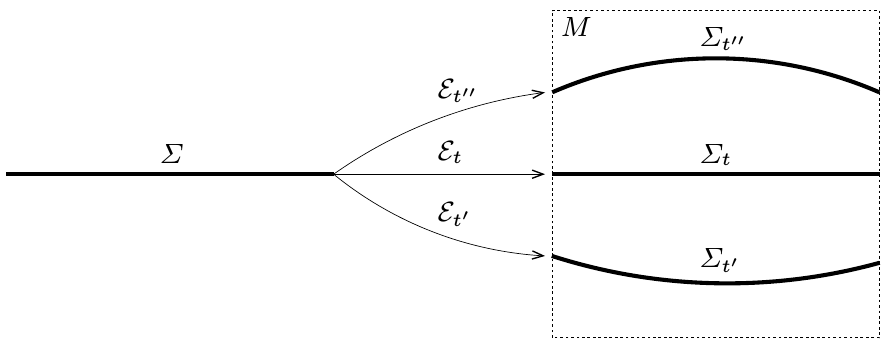
\includegraphics[width=0.85\textwidth]{FoilM.png}
\caption{Separación de la variedad $M$ mediante una familia, de un único parámetro, de encajes $\varepsilon_t$ de 3-variedades $\Sigma$ en $M$. $\Sigma_t$ es la imagen en $M$ de $\Sigma$ bajo $\varepsilon_t$.}
\label{fig:FoilM}
\end{figure}


Supongamos que tenemos una estructura de espacio-tiempo, es decir, una variedad diferenciable $M$ de dimensión cuatro y métrica $g_{\mu\nu}$ que se puede <<separar>> mediante una familia $\{\Sigma_t\,|\,t\in\mathbb{R}\}$ de hojas espaciales (hipersuperficies espaciales). Es decir, que para número $t$ existe un <<encaje>> (\emph{embedding}) de una variedad fija $\Sigma$ de imensión tres en $M$
\begin{equation*}
 \varepsilon_t\,:\,\Sigma\rightarrow M\,,
\end{equation*}
cuya imagen $\varepsilon_t(\Sigma)\subset M$ es $\Sigma_t$, una subvariedad de la variedad $M$. En la figura (\ref{fig:FoilM}) se muestra este procedimiento. Cada hoja tridimensional $\Sigma_t$ se corresponde con un instante de tiempo $t$, donde $t$ es un <<tiempo>> topológico, una forma de etiquetar los instantes de forma continua pero que no tiene nada que ver con el tiempo de los relojes.

Gracias a este mecanismo hemos logrado recuperar la noción de tiempo: podemos ver el espacio-tiempo ($M,g$) como una familia de espacios parametrizada por un único parámetro $t$. De esta forma, el espacio-tiempo se interpreta como una <<trayectoria de espacios>> tridimensionales. La ecuaciones de Einstein que vimos en clase
\begin{equation*}
 G_{\mu\nu}=-8\pi GT_{\mu\nu}
\end{equation*}
en las que no se podía plantear un problema de valor inicial quedarían reformuladas en forma de una ecuación de evolución en la que dada la geometría de una hipersuperficie (valor inicial) podríamos determinar cómo evolucina esta geometría a lo largo del <<tiempo>>.

Esta forma de plantear el problema induce unas ligaduras conectadas con las invariancias de la teoría. De esta forma, uno tiene cuatro ligaduras locales asociadas con los difeomorfismos\footnote{Un difeomorfismo \cite{difeomorfismo} es un mapeo entre variedades, que es diferenciable y tiene un inverso también diferenciable.} clásicos: una es la ligadura del Hamiltoniano $\mathscr{H}_\perp$, la cual genera deformaciones en las hipersuperficies; las tres restantes serían las ligaduras del momento o las ligaduras $\mathscr{H}_a$, las cuales generan transformaciones de las coordenadas tridimensionales. En clase sólo hemos trabajado con la conexión de Levi-Civita, pero en realidad ni siquiera estamos limitado a trabajar con variedades riemannianas. Una teoría muy usada en física teórica es la teoría de las tétradas o \emph{Vierbeins}, que es un caso especial de aplicación de la conexión de Cartan en variedades cuadridimensionales. En esta situación surgirían tres ligaduras adicionales, que reciben el nombre de ligaduras de Gauss, y que estarían asociadas con la libertad de realizar transformaciones de Lorentz locales.

Mediante la cuantización, estas ligaduras clásicas se transforman en ligaduras cuánticas para las funciones de onda válidas. La forma exacta depende de cómo escojamos nuestras variables canónicas. Esto da lugar a la dos ramas dentro de los intentos canónicos de cuantizar la gravedad: la geometrodinámica y la gravedad cuántica de bucles.


\subsection{\textit{Quantum Geometrodynamics}}

\textit{Quantum Geometrodynamics}, gravedad cuántica geometrodinámica o, simplemente, geometrodinámica es una de las formas en las que se ha intentado cuantizar la gravedad. Esta teoría fue introducida por Arnowitt, Deser y Misner en los años 60, y también muy promovida por John Wheeler.

En geometrodinámica, las variables canónicas son la métrica $g_{\mu\nu}$ y sus momentos canónicamente conjugados $\pi^{\sigma\tau}$. Estas variables se convierten en operadores de forma análoga a cómo lo hacen los operadores posición y momento habituales usando las reglas de conmutación

\begin{equation*}
 \Big[\hat{g}_{\mu\nu}(x),\hat{\pi}^{\sigma\tau}\Big]=i\hbar\,\tensor{\delta}{^\sigma}{_\mu}\tensor{\delta}{^\tau}{_\nu}\delta(x,y)
\end{equation*}

Usando un procedimiento sugerido por primera vez por Dirac, las ligaduras clasicas se implementan como ligaduras cuánticas, como dijimos antes, en las funciones de onda

\begin{align*}
 \mathscr{H}_\perp\Psi&=0\\
 \mathscr{H}_a\Psi&=0
\end{align*}

La primera ecuación se conoce como la \textbf{ecuación de Wheeler-DeWitt} y las otras tres simplemente se llaman ligaduras del momento. Estas tres ligaduras garantizan que la función de onda sea invariante bajo transformaciones de coordenadas. Las ecuaciones de vacío tomarían la siguiente forma

\begin{align*}
  \mathscr{H}_\perp\Psi\equiv\Big(-16\pi G\hbar^2G_{\mu\nu\sigma\tau}\frac{\delta^2}{\delta g_{\mu\nu}\delta g_{\sigma\tau}}-\frac{\sqrt{g}}{16\pi G}(R-2\Lambda)\Big)\Psi&=0\\
 \mathscr{H}_a\Psi\equiv-2D_\nu h_{\mu\sigma}\frac{\hbar}{i}\frac{\delta\Psi}{\delta g_{\nu\tau}}&=0\,,
\end{align*}
donde $D_\nu$ es la derivada covariante y $G_{\mu\nu\sigma\tau}$ es la métrica de DeWitt.

Uno de las primeras formulaciones hamiltonianas de la relatividad general de este estilo se conoce como el formalismo ADM (por las iniciales de Arnowitt, Deser y Misner). Sin embargo, Wheeler quería reducir la física de una manera más fundamental que la ADM. Wheeler, en oposición a la visión de Weinberg que hemos podido ver en su libro, quería reducir toda la <<física>> a la geometría del espacio-tiempo, una geometría dinámica que fuera evolucionando y que explicara la masa, la carga eléctrica y los campos sin masa, cargas ni campos, de forma puramente geométrica. La base de su gravedad cuántica era tratar de unificar la gravedad y el electromagnetismo, ya que por aquella época las fuerzas fuerte y débil aún no se entendían demasiado bien. Llegó a introducir la noción de \textbf{\emph{geons}} (término que se obtiene de contraer <<\emph{gravitational electromagnetic entity}>>), unos paquetes de onda gravitacional confinados en regiones compactas del espacio-tiempo y que se mantenían nudios por efectos gravitacionales debidos a la energía del campo gravitatorio creado por la propia onda. Realmente, los \emph{geons} de Wheeler no eran entidades cuánticas pero sí que especuló acerca de una posible relación con las partículas elementales. Tampoco llegó a presentar soluciones a la ecuación de vacío de Einstein. Fue años después, en 1997, cuando Anderson y Brill \cite{geons} dieron una demostración rigurosa de que los \emph{geons} eran una solución existente para las ecuaciones de vacío de Einstein.

Los \emph{geons} siguen llamando la atención hoy en día entre algunos físicos y aún hay muchísimas preguntas sin responder como por ejemplo si son estables o si, por el contrario decaen a medida que la energía de la onda se escapa. De todas formas, a día de hoy no hay ninguna forma de testear la validad de esta idea. Heredando algunos de los objetivos que se había planteado Wheeler (masa sin masa, carga sin carga, \dots), las investigaciones por estos intentos de cuantizar la gravedad están liderados por Christopher Isham y Jeremy Butterfield junto a sus estudiantes.

\subsection{\textit{Loop Quantum Gravity}}

La gravedad cuántica de bucles (\textit{Loop Quantum Gravity}) es un enfoque canónico no perturbativo de la teoría de la gravedad cuántica en la que no se utiliza ninguna métrica clásica. El punto de partida tampoco es una linealización de la teoría de la relatividad general sino que utiliza variables conceptualmente más próximas a las que aparecen en teoría de Yang-Mills, esto es, teorías de gauge basadas en los grupos especial unitarios $SU(N)$ que tratan de explicar el comportamiento de las particulas elementales mediante grupos de Lie no conmutativos\footnote{Por ejemplo, la cromodinámica cuántica, la teoría de la interacción fuerte o de color se basa en el grupo $SU(3)$.}, la base del modelo estándar.

En estas teorías el propio espacio está cuantizado, se habla de un espacio granulado, un espacio constituido por  un tejido de lazos finitos. Estas redes de \emph{loops} reciben el nombre de redes de espín, mientras que cuando se estudia la evolución de las redes de spin con el tiempo se habla de la \emph{spin foam} o espuma de espín. El tamaño que predicen estas teorías para estas estas estructuras es del orden de la escala de Planck, es decir, $\sim\SI{e-35}{m}$. Esta sería la longitud mínima, es decir, que no solo la matería estaría constituida por entidades fundamentales sino que el propio espacio sería discreto y tendría una distancia mínima.

Hoy en día, es una de las ramas de la gravedad cuántica en las que más se investiga, con alrededor de 30 grupos de investigación por todo el mundo. Aunque todos los grupos parten de unas suposiciones comunes se pueden distinguir dos direcciones: el planteamiento más tradicional que sería la gravedad cuántica de bucles canónica, y por otra parte la más reciente versión covariante, que suele recibir el nombre de \emph{spin foam theory}. La principal diferencia de la gravedad cuántica de bucles frente a otros enfoques como puede ser la teoría de cuerdas, de la que hablaremos a continuación, es que <<no apunta tan alto>> en el sentido de sus aspiraciones como teoría. No pretende una gran unificación basándose en alguna simetría más general o en alguna reformulación más profunda de las reglas de la teoría cuántica de campos, sino que <<simplemente>> pretende cuantizar la teoría de Einstein en cuatro dimensiones.

En definitiva, \textit{Loop Quantum Gravity} es una teoría cuántica de campos muy inusual, una teoría muy prometedora para tratar de unificar la relatividad general y la teoría cuántica, que ya ha dado algún que otro fruto, sobre todo en el ámbido de la cosmología (\emph{loop quantum cosmology}). El resultado más espectacular ha sido el poder estudiar la evolución del universo más allá del Big Bang, que ha dado lugar a un nuevo modelo hipotético que sustituiría al Big Bang: el Big Bounce, un modelo cicliclo en el que el Big Bang no sería más el resultado del colapso de un universo previo al nuestro.

%
%
%
%
\newpage
\section{Teoría de cuerdas}

De entre todas las propuestas para resolver el dilema, existe una de las principales que es completamente distinta al resto. Su diferencia radica en la forma de enfrentar el problema, que es cualitativamente distinta. Mientras que, más o menos, el resto de teorías parten de las ideas bien asentadas de bien relatividad general, o bien de la teoría cuántica, «salvando los trastos», la teoría de cuerdas no. Digamos que «echa la casa por la ventana» (y se construye otra).

Esta teoría surgirá gracias a un grupo de trabajo comenzado por Werner Heisenberg en 1943, basado en el estudio de una teoría denominada teoría de la matriz S (\textit{S-matrix theory}), y durante lo que queda de siglo (estrictamente hablando de teoría de cuerdas, de los 60' en adelante) se consolidaría como un referente de estudio en la física teórica. Además, se convertirá en motivo de discusión casi omnipresente en toda la comunidad científica, incluso entre no físicos. Veamos el porqué.

La teoría de cuerdas \textit{no busca} la reunificación de la relatividad general con la teoría cuántica. Este modelo teórico ofrece una explicación a los cuatro tipos de interacciones entre partículas elementales a través de su \textbf{concepto esencial}: la \textbf{reinterpretación de las partículas elementales como modos de vibración de un nuevo ente elemental que «vive» en más dimensiones que nuestras cuatro}. Y estos entes elementales nuevos son \textit{cuerdas}: cuerpos unidimensionales caracterizados tan solo por un parámetro dimensional, o longitud de la cuerda. Bajo este marco, la cuantización de la gravedad aparece como un resultado de la teoría, de forma completamente natural. Es más, la propia gravedad aparece \textit{per se}: la partícula que la media, el gravitón, es un modo de resonancia de las cuerdas cerradas.\footnote{Lo que posibilida una conexión con las teorías covariantes de gravedad cuántica.} Hay que hacer constar que las cuerdas no son los únicos objetos que pueden existir, según los resultados formales. Otros entes como d-branas coexisten con ellos: son cuerpos d-dimensionales. Además, las dimensiones extra en las que las cuerdas o las d-branas pueden vivir no son cualesquiera: responden a restricciones que se deben de hacer sobre algunos elementos de la teoría.

Pese a que resuelve la mezcla entre física cuántica y gravedad einsteiniana, no arregla todos los problemas: \textbf{no es \textit{background independent}}, aunque se sabe que bajo las teorías de cuerdas con la conjetura AdS/CFT (anti-de Sitter/\textit{Conformal Field Theory}\footnote{Vinculadas con la teoría de cuerdas desde 1997, la conjetura AdS/CFT es un campo hoy en día en estudio en la física teórica. Dentro de \textit{String Theory}, permitirían la reinterpretación de la gravedad en nuestro espacio-tiempo respecto de otra teoría más general de igual modo que un holograma nos ofrece información en varias dimensiones de algo que es real.}) actualmente en desarrollo se podría obtener una independencia \textit{parcial} del fondo. Hemos de hacer notar que no existe \textit{una} teoría de cuerdas, se trata más bien de un paradigma, y los modelos de \textit{String Theory} se dividen en distintas aproximaciones, entre las cuales destaca la teoría M (de 11 dimensiones), de la que se probó su particularización a otras teorías anteriores.

Aunque existe un bache con la independencia de fondo, la teoría de cuerdas ofrece muchas interpretaciones novedosas que sobre el papel solucionan muchos problemas actuales de la física. Es más, algunos físicos teóricos afirman que más que otra cosa, ofrece \textit{ideas}. Gracias a ella, por ejemplo, y al desarrollo de teorías con conjetura AdS/CFT, se pudo encontrar la aplicación de la conjetura en materia condensada. Otros casos de este tipo aparecen por el lado de la matemática, como es la investigación en simetría especular. En resumidas cuentas, la teoría de cuerdas \textbf{sería} una posible explicación mucho más profunda y revolucionaria, no sólo de la gravedad cuántica, sino de toda la física en general. Incorporaría los resultados del modelo estándar, de la relatividad general y se erigiría como candidata a teoría del todo (TOE, \textit{Theory of Everything}), aunque hay debate sobre este asunto. Es posible que se haya dado cuenta de que este párrafo está todo escrito en condicional. No es coincidencia: el motivo de ese tiempo verbal es en verdad la fuente de toda \textbf{la discordia con la teoría de cuerdas}.

Durante los últimos años, es difícil encontrar una universidad con departamento de física o de física teórica en el que no se trabaje, en mayor o menor grado, en teoría de cuerdas. Esto es prueba de la gran presencia que tiene en la física teórica actual. Sin embargo, ello no quita que sea objeto de una fuerte polémica. El origen de la misma es que la teoría de cuerdas, pese a haber tenido mucho desarrollo desde sus inicios allá a mediados del siglo anterior, \textbf{carece de predicciones que puedan ser comprobadas experimentalmente en la actualidad}: no es falsable. Y, por tanto, según los estándares de la ciencia, la teoría de cuerdas, no es una teoría \textit{científica} en el sentido en el que lo son la relatividad general, la especial, o la mecánica cuántica\footnote{Entiéndase esta «definición» (no pretende serlo en verdad) en sentido amplio.}. Esto hace que, en según qué grupos de científicos, sea posible distinguir claramente dos bandos: aquellos que apoyan la investigación en teoría de cuerdas en mayor o menor grado y los que discrepan de la misma de igual modo.

Otra forma de ver el problema de la falta de predictibilidad nos la comenta Kiefer (\cite[p.~8]{paper_osorio}). De acuerdo con la teoría, no sería descabellado pensar que la realidad posee un guarismo elevadísimo ($\approx10^{500}$) de estados de mínima energía. Al parecer, la selección sólo parece posible a partir del principio antrópico, de modo que no existe predictibilidad en tal elección por parte de la teoría de cuerdas.

Debido al potencial que muchos ven en la teoría de cuerdas, muchos físicos invierten sus esfuerzos en encontrar algún tipo de predicción que la pueda poner a prueba. Sin embargo, no es para nada tarea fácil. Comentaremos algunas de las posibilidades que existen a este respecto en la sección de cosmología cuántica, particularmente la boyante cosmología de cuerdas, o \textit{string cosmology}.

\begin{figure}[h]
	\centering
	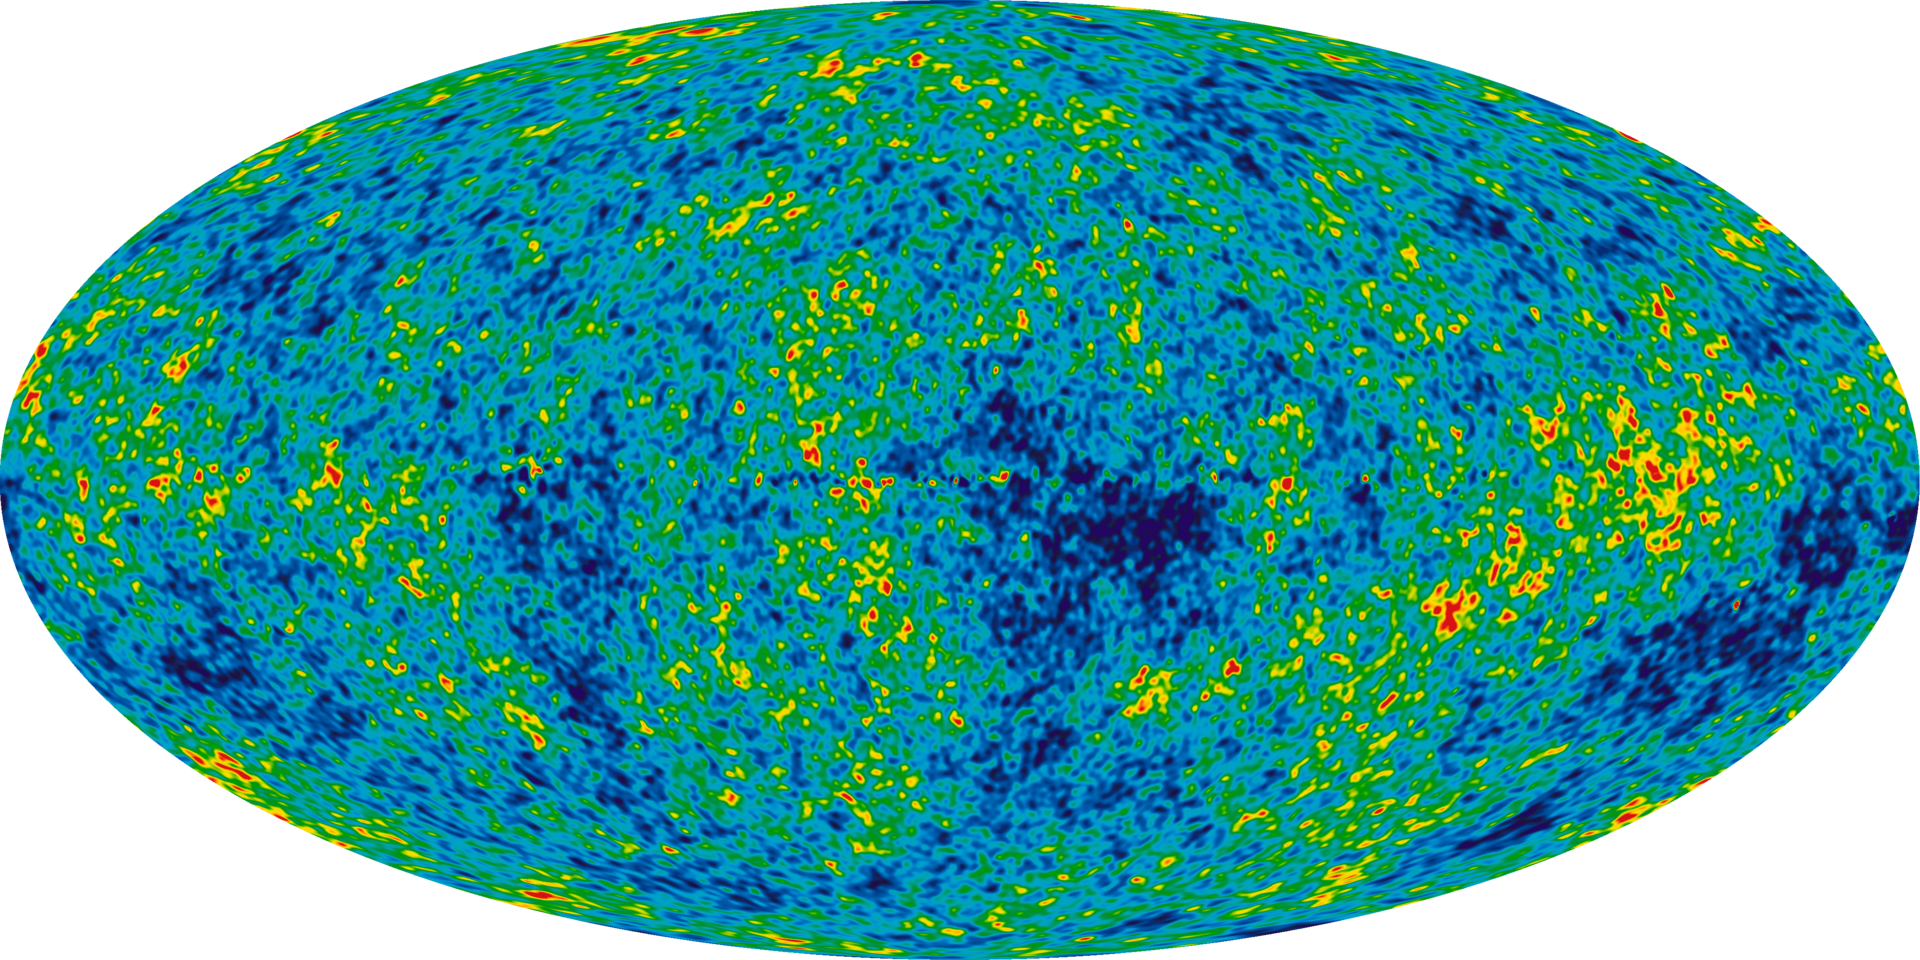
\includegraphics[width=0.8\textwidth]{cmb}
	\caption{\cite{cmbbib}. Señal de fondo cósmico de microondas (CMB) recopilada por el satélite WMAP. Se espera que la cosmología cuántica de cuerdas permita nuevas interpretaciones del cosmos a gran escala y, quizás, que dé alguna predicción que pueda ser contrastada con la realidad.}
	\label{cmb}
\end{figure}

%
%
%
%
\newpage
\section{Teorías de campo efectistas} % Víctor

Aparte de las teorías que se enfrentan al problema con ánimo de resolverlo completamente, existe quien, quizás debido a la dificultad del problema, prefiere \textbf{aproximar resultados}. Para ello, las teorías de campo efectistas son una solución. En esencia, y de forma resumida, las teorías de campos efectistas se basan en una aproximación en la que, para un determinado intervalo de energías es posible obtener unos resultados despreciando valores que no son importantes en ese intervalo. Lo que se hace es escoger los grados de libertad que nos interesan para nuestro intervalo de energías, excluyendo aquellos que se alejen de él. Estas teorías no son esencialmente gravitatorias, sino que ya se han usado en otras ramas de la física con éxito, como en superconductividad (materia condensada) o física de partículas.

No es una idea nueva: desde los 80' rondaba por los salones de la física teórica ésta forma de actuar, pero en los años del último siglo se le ha dado un nuevo empujón. Las diferencias esenciales con el resto de aproximaciones generales no sólo están en que los resultados son aplicables a determinados intervalos de energía (otras teorías también dan algunos resultados aproximados), sino que ofrece un modo de calcular a través de un proceso sistemático estos resultados, y también posibles nuevas predicciones.

El interés de las \textit{effective field theory} para la gravedad cuántica radica en una propiedad muy interesante que poseen: no necesitan que la teoría, que los desarrollos, sean no renormalizables para que se pueda aplicar. Sabiendo ésto, parece claro que la gravedad cuántica podría ser un sujeto válido, teniendo en cuenta una cosa más: los resultados a los que la teoría efectista gravitocuántica podría llegar tendrían que ser en un régimen de energías no alto. Es decir, no serían válidos a cortas distancias y el motivo es evidente: se espera que ahí sea cuanto los efectos cuánticos sean más notorios. Entonces, las aproximaciones que la teoría ofrezca no serán válidas.

Pese a que ya dijimos que este modelo tiene alguna que otra presencia desde el siglo XX, es ahora cuando está teniendo un resurgir. Además, de acuerdo con Burgess, mucho trabajo está por hacer en esta aproximación a teorías de gravedad cuántica. Las predicciones (correcciones cuánticas) de momento son de un orden de magnitud no medible, pero la esperanza es que en el futuro esto cambie. Además de que nuevos campos hoy en estudio podrían ser interesantes para la teoría (cosmología cuántica).

%
%
%
%
\newpage
\section{Otras aproximaciones} % Tú o yo

Hemos comentado ya las propuestas mayoritarias para cuantizar la gravedad pero, como dijimos al principio, un problema de este calado ha tenido una repercusión tal que son \textit{bastantes} las teorías de gravedad cuántica que han sido presentadas. No daría tiempo aquí a tratarlas todas, pero comentaremos algunas generalidades.

Un ejemplo de estos modelos es la \textbf{teoría de sistemas causales fermiónicos}. Procedente de teoría cuántica de campos, es una apuesta para describir una física más fundamental a ésta y a la teoría de la relatividad general, surgiendo éstas como casos límites de la misma. Es más, bajo este paragüas, ¡incluso el espaciotiempo surge, y no necesita ser impuesto! En esencia, consiste en deducir los conocimientos asentados a partir del marco de un sistema causal de fermiones.

Una explicación más es, por ejemplo, la \textbf{gravedad cuántica euclidiana}. Ésta se basa en encontrar soluciones a problemas dinámicos en $n$ dimensiones llevándolos a $n+1$ dimensiones a través de una transformación que se llama rotación de Wick. Los números complejos aparecen en escena como actores casi principales en éste modelo.

La teoría de tuistores (\textbf{\textit{twistor theory}}) se basa en encuadrar, también con ayuda de números complejos, el espacio de Minkovski 3+1 en un espacio 4-dimensional con signatura métrica (2,2). De este modo, constituye una generalización de la teoría de espinores de Dirac. Ha sido aplicada a teoría cuántica de bucles y a teoría de cuerdas.

Otras propuestas vienen de la mano de la física estadística, como la teoría del vacío de superfluido (\textbf{\textit{superfluid vacuum theory}}). Este modelo constituye una aproximación a la gravedad cuántica a través de uno de sus elementos más notorios: el vacío. Lo que hace la teoría es reinterpretarlo bien como un superfluido o como un condensado de Bose-Einstein. Dentro de este marco existen varias subteorías de vacío de superfluido, que se diferencial principalmente en las propiedades del superfluido.

Como vemos, existen muchas candidatas a resolver el dilema de la gravedad cuántica, aparte de la teoría de cuerdas, la teoría de \textit{loops}... También hay algunas ideas que no llegan a la categoría de teoría propiamente dicha, pero que resultan útiles a los modelos grandes. Por ejemplo: \textbf{la métrica acústica}. Se postula que las singularidades derivadas de su estudio son interpretaciones análogas a un agujero negro convencional.

%
%
%
%
\newpage
\section{Cosmología cuántica}

La cosmología cuántica es la aplicación de las teorías cuánticas de la gravedad para estudiar el universo como un todo. Conceptualmente, esto se corresponde con el problema de formular la teoría cuántica para un sistema cerrado desde dentro de él, sin ninguna referencia a observadores externos ni mediciones. Esta formulación va a requerir la cuantización de la gravedad ya que es la fuerza que predomina a estas escalas. Además, desde la relavitidad general sabemos que el espacio-tiempo juega el papel de un objeto físico más y su cuantización es por tanto necesaria. Por una parte, la cosmología cuántica puede ofrecer formas de testear las teorías cuánticas de la gravedad en configuraciones matemáticamente más simples, y por otra parte también puede tener mucho que decir acerca de la comprensión de nuestro universo.

Hay muchas formulaciones de la cosmología cuántica, en principio tantas como formulaciones de la gravedad cuántica haya, y por eso se puede encontrar gente que dedica su tiempo a cosmología cuántica supersimétrica, cosmología cuántica de bucles, \emph{string quantum cosmology}, cosmología cuántica no conmutativa, etc.. La mayor parte de las versiones de cosmología cuántica toman como punto de partida clásico la relatividad general de Einstein.

En este apartado sólo queremos mostrar una idea global sin decantarnos por ninguna rama en particular. La cosmología cuántica normalmente se plantea para modelos homogéneos y en la formulación más sencilla también se asume la isotropía. En una configuración en la que que se tiene en cuenta la presencia de materia, se añade un campo escalar $\phi$ con un potencial $V(\phi)$ y la ecuación de Wheeler-DeWitt se convierte en una ecuación de derivadas parciales bidimensional

\begin{equation*}
 \Bigg[\frac{\hbar^2\kappa^2}{2}a\frac{\partial}{\partial a}a\frac{\partial }{\partial a}-\frac{\hbar^2}{2}\frac{\partial^2}{\partial\phi^2}+a^6\Big(V(\phi)+\frac{\Lambda}{\kappa^2}\Big)-\frac{3ka^4}{\kappa^2}\Bigg]\Psi(a,\phi)=0
\end{equation*}

donde $\kappa\equiv8\pi G$, $a$ viene del elemento diferencial $ds^2=-N(t)^2dt^2+a(t)^2d\Omega_3^2$, $k$ sería el índice de curvatura espacial ($k=0,\pm1$) y $\Lambda$ la constante cosmológica. Se puede definir una nueva variable $\alpha\equiv\ln a$ y reescribir la ecuación anterior con la ventaja de que la nueva variable tiene un rango desde $-\infty$ a $+\infty$.

\begin{equation*}
 \Bigg[\frac{\hbar^2\kappa^2}{12}\frac{\partial^2}{\partial\alpha^2}+\frac{\hbar^2}{2}\frac{\partial^2}{\partial\phi^2}+e^{6\alpha}\Big(V(\phi)+\frac{\Lambda}{\kappa^2}\Big)-3e^{4\alpha}\frac{k}{\kappa^2}\Bigg]\Psi(\alpha,\phi)=0
\end{equation*}

En el caso de cosmología cuántica por bucles, la ecuación que se plantean difiere de esta última pero a escalas más alla de la longitud de Planck las diferencias entre ambas ecuaciones desaparecen. En cualquier caso, en ambos planteamientos, las ecuaciones diferenciales son difíciles de resolver así que \textbf{al final se recurre a teorías efectivas}. Muchas de las características que presenta la cosmología cuántica se estudian en el límite cuando la ecuación de Wheeler-DeWitt toma la forma WKB\footnote{La aproximación o método WKB (por las iniciales de Wentzel, Kramers y Brillouin) es un método para encontrar soluciones aproximadas a ecuaciones diferenciales lineales con coeficientes espaciales variables. Es un método habitualmente usado para cálculos semiclásicos en mecánica cuántica en la que la función de onda se escribe como una función exponencial, se exande semiclásicamente, y luego se varía lentamente o bien la amplitud o bien la fase.}. Incluso se ha llegado a plantear que la función de onda del universo sólo puede ser interpretada en el límite WKB porque sólo en esos casos aparece el parámetro tiempo y una ecuación similar a la de Schrödinger. Además de que conceptualmente esto conlleva muchas dudas y, por tanto, el mayor número posible de implicaciones del significado de las funciones de onda en cosmología cuántica se deberían derivar de las soluciones exactas y no de esta aproximación, el límite WKB falla en muchas situaciones interesantes.




%
%
%
%
\newpage
\section{Conclusiones y perspectivas de futuro} % ¿Los dos?

Durante los últimos 70 años (aprox.) la ciencia ha tratado de encontrar un modelo que englobe la teoría de la relatividad general y la física cuántica para solucionar algunos problemas que existen en el marco actual. En este tiempo la tecnología y la física teórica han avanzado de modo que tenemos modelos teóricos cada vez más refinados con predicciones más precisas, e instrumentos de observación mejores, que aumentan también la precisión experimental.

En este sentido, \textbf{todos los \emph{tests} que se han realizado a la relatividad general de Einstein en los escenarios más extremos conocidos} (y observables), que son los púlsares binarios y en concreto el púlsar doble \texttt{PSR J0737-3039} descubierto en 2003, \textbf{han confirmado las predicciones de la teoría}. Así mismo, la \textbf{teoría cuántica sigue estando firmemente asentada bajo numerosas pruebas experimentales}.

\textbf{El problema del descubrimiento podrían ser nuestras limitaciones tecnológicas}. Quizás con nuevas generaciones de radiotelescopios (ALMA, SKA, Euclid, SNAP, etc.), al aumentar la nitidez y resolución de las medidas, se observen desviaciones entre teoría y naturaleza, y esto arroje algunas pistas acerca del camino correcto en el laborioso trabajo de cuantizar la gravedad. Tal vez las futuras mediciones no hagan más que validar de nuevo la teoría de Einstein y entonces las comprobaciones experimentales de la cuantización de la gravedad tengan que venir de otro sitio (¿quizás de la mano de aceleradores de partículas?).

Además, las últimas observaciones experimentales, por ejemplo, en supernovas no han hecho sino confirmar más misterios como la energía oscura que deberán ser explicados por estas nuevas teorías. Es más que posible que los nuevos experimentos arrojen nuevas pistas, pero también nuevas preguntas.

En cualquier caso, \textbf{la cuantización de la gravedad parece lejos aún de conseguirse satisfactoriamente}, y quizás su realización requiera de alguna \textit{mente privilegiada} al igual que ocurrió con la teoría de la relatividad general.

En este sentido, y con cada nuevo dato experimental, los modelos sufren, se alegran, o se adaptan. La problemática de la teoría de cuerdas, salvo que se consigan progresos en la obtención de datos firmemente experimentales está servida en el futuro cercano. Esto posiblemente aliente nuevos acercamientos más proclives a ofrecer un contacto \textit{rápido} con la realidad, como los efectistas. Y \textbf{uno de los campos seguro a tener en cuenta es el de la cosmología cuántica}. Los últimos cuarenta años han sido una época de oro de la cosmología, y por lo que llevamos visto, tendrá un papel importante en la física teórica de los próximos lustros.

Lo que no se puede dudar es que \textbf{el problema de la cuantización de la gravedad sigue siendo, y será (por el momento) uno de los mayores dilemas de la física y la ciencia en general}.

%
%
%
%
\newpage
\section{Bibliografía}
\bibliographystyle{ieeetr}
\bibliography{Referencias}
\nocite{*}

\end{document}
